\section{Experimental Results}
For our evaluation, we implemented PC extractor module at the 
system call layer 
and the lifetime analyzer and stream mapper module 
at the block device layer in the Linux kernel version 4.5.
We also implemented manual technique~\cite{MultiStream}, 
Autostream~\cite{AutoStream}, and
baseline which uses only one stream.
to compare them with {\sf PCStream}.
For a detailed analysis, {\sf PCStream} is also compared to {\sf PCStream}$^{--}$
which excludes the second phase substream assignment 
to see the effectiveness PC-based data separation only.

In order to evaluate the effectiveness of {\sf PCStream},
we conduct experiments on two enviroments; the first one is 
for the emulation.
We implemented the multi-stream feature and substream concept
to the in-house SSD emulator
based on the open flash development platform~\cite{AMF}.
The number of streams was set to 8 for the evaluation.
The SSD emulator was 12 GB with four channels with four ways, and 
the number of blocks per parallel unit was 512 and
the number of pages per block was 384 with page (4 KB).
Due to the limited capacity of the emulator, 
we scaled down the configuration of RocksDB.
The base file size is set to 8 MB
with an key-value pair (8 KB) and the number of levels was set to 4.
However, the size of level multiplier is remained to be 10 as the general setting,
which means the size of the next level is 10 times larger than the previous level,
to maintain the level access patterns during the compaction.

The second one is for Samsung PM963 480GB SSD (with 8 streams).
As a warming workload, we wrote a single file sequentially to fill 90\%
of logical device capacity, to ensure that 90\% of logical space stays valid
throughout the test.

For benchmarks, we used three scenarios of db\_bench of RocksDB.
The first one is the update random scenario, {\tt UR}, which read-modify-writes for random keys. 
The second one is append random scenario, {\tt AR}, which read-modify-writes with growing values.
The last one is the fill random scenario, {\tt FR}, which writes values in random key order and 
shows higher write ratio than others.
The number of keys were set to about 900,000 for the emulator and about 90,000,000 for
the SSD.

\subsection{Results on the SSD emulator}

\begin{figure}[t]
	\centering
	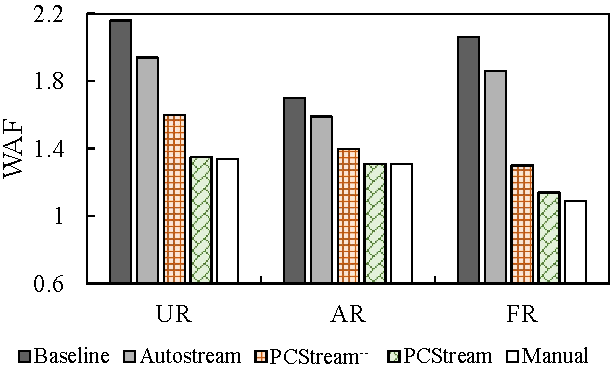
\includegraphics[width=1\linewidth]{figure/result_emul.pdf}
	\vspace{-15pt}
%	\caption{The WAF comparison on the emulator.}
	\caption{A comparison of WAF on the SSD emulator.}
	\label{fig:result_emul}
	\vspace{-15pt}
\end{figure}

We compared WAF of the existing techniques with {\sf PCStream}
for each scenario and the result is shown in Fig.~\ref{fig:result_emul}. 
As shown in Fig.~\ref{fig:result_emul}, 
{\sf PCStream}$^{--}$ reduces WAF by 25\% on average over the AutoStream. 
The result shows that separating short-lived data such as log or flush
using PC was quite effectvive in reducing WAF.
Moreover, {\sf PCStream} showed similar WAF to the manual technique,
reducing WAF by 30\% on average
over the AutoStream.
The additional benefit comes from separating
long-lived data of the compaction PC during the
second phase assignment.

\subsection{Results on Samsung PM963 SSD}
\begin{figure}[t]
	\centering
	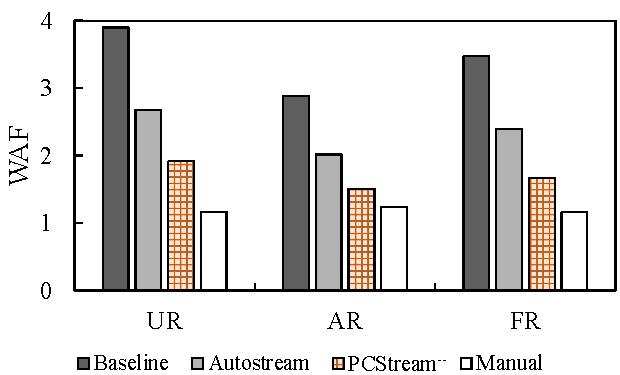
\includegraphics[width=1\linewidth]{figure/result_ssd.pdf}
	\vspace{-15pt}
	\caption{A comparison of WAF on PM963.}
	\label{fig:result_SSD}
	\vspace{-15pt}
\end{figure}

%Since we can not implement the second-phase substream assignment for the SSD, 
We evaluated the efficiency of {\sf PCStream} on real SSDs using Samsung PM963 SSDs with 8 streams.  
Since it was not possible to modify the PM963's firmware, 
we used {\sf PCStream}$^{--}$ in our evaluation.
%we compare {\sf PCStream}$^{--}$ only for the SSD.
As shown in Fig.~\ref{fig:result_SSD}, 
{\sf PCStream}$^{--}$ reduces the average WAF by 26\% over AutoStream. 
There exists large WAF gaps between {\sf PCStream}$^{--}$ and the manually optimized case. 
However, if the substream is properly supported during garbage collection, 
we believe that {\sf PCStream} can similar WAF vlaues as the manual case. 
Although {\sf PCStream}$^{--}$ still outperforms AutoStream, 
a performance gap is smaller over that in the emulated SSD environment. 
It is difficult to pinpoint why AutoStream works better in PM963 over in the emulated SSD, 
but we suspect that some internal features of PM963 such as a large block size or some implementation details of streams might be related. 
%Although AutoStream on the SSD works better than on the emulator, {\sf PCStream}$^{--}$ still outperforms AutoStream, thus showing the effectiveness of the PC-based data separation.
%If the program is written in more PC-friendly manner, {\sf PCStream} will be able to get closer WAF to manual.

